\documentclass[tikz,border=0pt]{standalone}
\usepackage{amsmath}
\usepackage{tikz}
\usetikzlibrary{arrows.meta,calc,patterns,decorations.pathmorphing}
\begin{document}
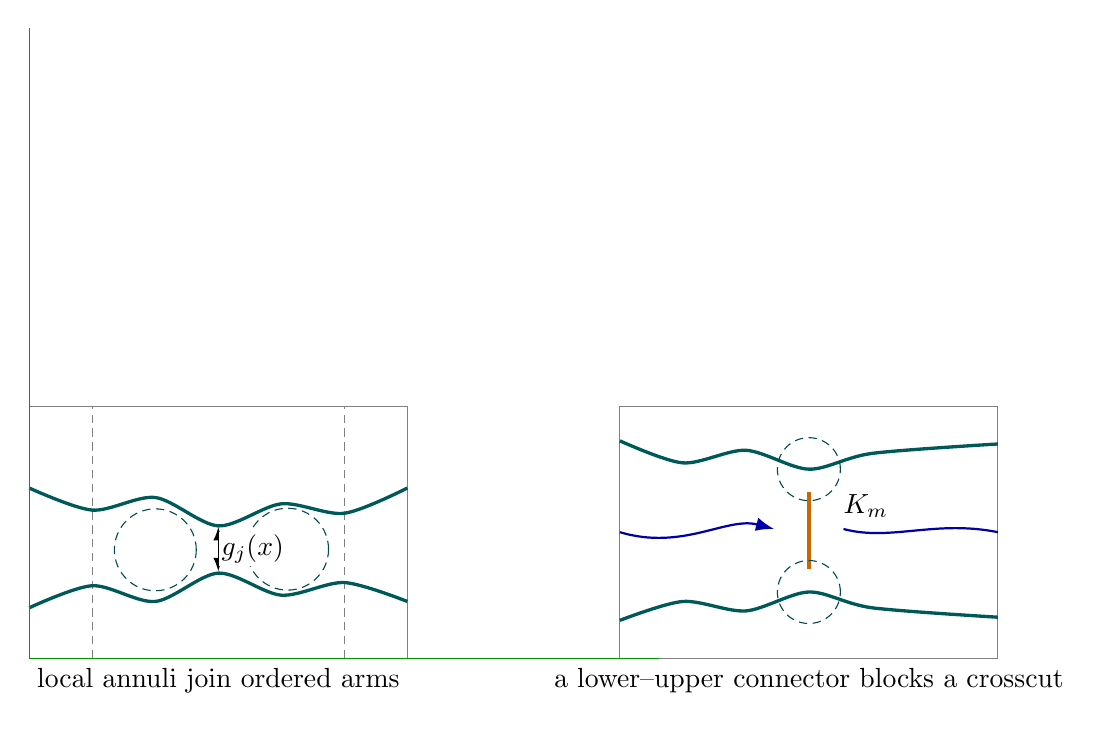
\begin{tikzpicture}[x=0.8cm,y=0.8cm,>=Latex]
 \draw[gray] (0,0) rectangle (6,4);
 \draw[densely dashed,gray] (1,0)--(1,4) (5,0)--(5,4);
 \draw[very thick,teal!70!black] plot[smooth] coordinates
   {(0,0.8) (1,1.15) (2,0.9) (3,1.35) (4,1.0) (5,1.2) (6,0.9)};
 \draw[very thick,teal!70!black] plot[smooth] coordinates
   {(0,2.7) (1,2.35) (2,2.55) (3,2.1) (4,2.45) (5,2.3) (6,2.7)};
 \draw[teal!60!black,densely dashed] (2,1.72) circle (0.65);
 \draw[teal!60!black,densely dashed] (4.1,1.73) circle (0.65);
 \draw[<->] (3,1.38)--node[right,fill=white,inner sep=1pt] {$g_j(x)$}
                  (3,2.08);
 \node at (3,-0.35) {local annuli join ordered arms};
 \begin{scope}[xshift=7.5cm]
  \draw[gray] (0,0) rectangle (6,4);
  \draw[very thick,teal!70!black] plot[smooth] coordinates
    {(0,0.6) (1,0.9) (2,0.75) (3,1.05) (4,0.8) (6,0.65)};
  \draw[very thick,teal!70!black] plot[smooth] coordinates
    {(0,3.45) (1,3.1) (2,3.3) (3,3.0) (4,3.25) (6,3.4)};
  \draw[very thick,orange!80!black] (3,1.42)--(3,2.63);
  \draw[teal!60!black,densely dashed] (3,1.05) circle (0.5);
  \draw[teal!60!black,densely dashed] (3,3.0) circle (0.5);
  \draw[blue!65!black,thick,->] (0,2.0).. controls (1.0,1.7) and
    (1.7,2.25)..(2.45,2.05);
  \draw[blue!65!black,thick] (3.55,2.05).. controls (4.3,1.85) and
    (5,2.2)..(6,2.0);
  \node[anchor=south west,inner sep=1pt] at (3.5,2.18) {$K_m$};
  \node at (3,-0.35) {a lower--upper connector blocks a crosscut};
 \end{scope}
\draw[green!60!black,line width=0.4pt] (0,0)--(10,0)(0,0)--(0,10);\end{tikzpicture}
\end{document}
